\section{Results}
We present results from running the adversarial scenarios in our approach for each of the research questions in the Sections below. 

\subsection{RQ1: Impact of Adversarial Generation on Threat Severity}
\begin{table*}[t]
\centering
\caption{Mean threat metric values across 30 scenarios per typology for seed (baseline near-miss) and generated (adversarial) scenarios using Baidu Apollo. Lower TTC, THW, and LTTC indicate greater risk; higher BTN and STN reflect greater risk. Bold values breach the emergency threshold (Table~\ref{tab:thresholds}).}
\label{tab:rq1_threat_comparison}
\renewcommand{\arraystretch}{1.0}
\begin{tabular}{@{}l cc cc cc cc cc@{}}
\toprule
& \multicolumn{2}{c}{\textbf{TTC [s] $\downarrow$}} & \multicolumn{2}{c}{\textbf{THW [s] $\downarrow$}} & \multicolumn{2}{c}{\textbf{BTN [--] $\uparrow$}} & \multicolumn{2}{c}{\textbf{LTTC [s] $\downarrow$}} & \multicolumn{2}{c}{\textbf{STN [--] $\uparrow$}} \\
\cmidrule(lr){2-3} \cmidrule(lr){4-5} \cmidrule(lr){6-7} \cmidrule(lr){8-9} \cmidrule(lr){10-11}
\textbf{Typology} & Seed & Gen. & Seed & Gen. & Seed & Gen. & Seed & Gen. & Seed & Gen. \\
\midrule
\rowcolor{blue!5}
(1) Lead Veh. Stopped         & 1.60 & \textbf{1.35} & 0.80 & \textbf{0.68} & 0.781 & \textbf{0.82} & -- & -- & -- & -- \\
\rowcolor{blue!5}
(2) Lead Veh. Decelerating    & 1.80 & \textbf{1.54} & 0.90 & \textbf{0.72} & 0.617 & 0.63 & -- & -- & -- & -- \\
\rowcolor{blue!5}
(3) Lead Veh. Lower Speed     & 2.40 & \textbf{1.54} & 0.60 & 0.77* & 0.174 & 0.63 & -- & -- & -- & -- \\
\rowcolor{green!5}
(4) Turning at Non-Signalized  & 1.54 & \textbf{1.20} & -- & -- & 0.63 & 0.60 & -- & -- & -- & -- \\
\rowcolor{green!5}
(5) Straight Crossing          & 1.80 & \textbf{1.20} & -- & -- & 0.46 & 0.70 & -- & -- & -- & -- \\
\rowcolor{green!5}
(6) LTAP/OD Signalized         & 2.10 & \textbf{1.44} & -- & -- & 0.322 & 0.68 & -- & -- & -- & -- \\
\rowcolor{green!5}
(7) LTAP/OD Non-Signalized    & 1.92 & \textbf{1.20} & -- & -- & 0.43 & 0.69 & -- & -- & -- & -- \\
\rowcolor{orange!5}
(8) Changing Lanes             & -- & -- & -- & -- & -- & -- & 1.40 & \textbf{0.48} & 0.279 & 0.689 \\
\rowcolor{orange!5}
(9) Turning Same Dir.          & -- & -- & -- & -- & -- & -- & 1.50 & \textbf{0.50} & 0.126 & 0.625 \\
\rowcolor{orange!5}
(10) Drifting Same Dir.        & -- & -- & -- & -- & -- & -- & 0.73 & \textbf{0.38} & 0.320 & \textbf{1.056} \\
\bottomrule
\end{tabular}
\end{table*}
% \begin{table*}[t]
% \centering
% \caption{Mean threat metric values across 30 scenarios per typology for seed (baseline near-miss) and generated (adversarial) scenarios using Baidu Apollo. Lower values of TTC, THW, and LTTC indicate a more safety-critical situation, whereas higher BTN and STN reflect greater risk.  Arrows indicate the direction of increased risk. Bold values denote metrics that breach the emergency threshold (Table~\ref{tab:thresholds}).}
% \label{tab:rq1_threat_comparison}
% \renewcommand{\arraystretch}{1.2}
% \begin{tabular}{@{}l cc cc cc cc cc@{}}
% \toprule
% & \multicolumn{2}{c}{\textbf{TTC [s] $\downarrow$}} & \multicolumn{2}{c}{\textbf{THW [s] $\downarrow$}} & \multicolumn{2}{c}{\textbf{BTN [--] $\uparrow$}} & \multicolumn{2}{c}{\textbf{LTTC [s] $\downarrow$}} & \multicolumn{2}{c}{\textbf{STN [--] $\uparrow$}} \\
% \cmidrule(lr){2-3} \cmidrule(lr){4-5} \cmidrule(lr){6-7} \cmidrule(lr){8-9} \cmidrule(lr){10-11}
% \textbf{Typology} & Seed & Gen. & Seed & Gen. & Seed & Gen. & Seed & Gen. & Seed & Gen. \\
% \midrule
% \rowcolor{blue!5}
% (1) Lead Veh. Stopped         & 1.60 & \textbf{1.35} & 0.80 & \textbf{0.68} & 0.781 & \textbf{0.82} & -- & -- & -- & -- \\
% \rowcolor{blue!5}
% (2) Lead Veh. Decelerating    & 1.80 & \textbf{1.54} & 0.90 & \textbf{0.72} & 0.617 & 0.63 & -- & -- & -- & -- \\
% \rowcolor{blue!5}
% (3) Lead Veh. Lower Speed     & 2.40 & \textbf{1.54} & 0.60 & 0.77* & 0.174 & 0.63 & -- & -- & -- & -- \\
% \addlinespace[4pt]
% \rowcolor{green!5}
% (4) Turning at Non-Signalized  & 1.54 & \textbf{1.20} & -- & -- & 0.63 & 0.60 & -- & -- & -- & -- \\
% \rowcolor{green!5}
% (5) Straight Crossing          & 1.80 & \textbf{1.20} & -- & -- & 0.46 & 0.70 & -- & -- & -- & -- \\
% \rowcolor{green!5}
% (6) LTAP/OD Signalized         & 2.10 & \textbf{1.44} & -- & -- & 0.322 & 0.68 & -- & -- & -- & -- \\
% \rowcolor{green!5}
% (7) LTAP/OD Non-Signalized    & 1.92 & \textbf{1.20} & -- & -- & 0.43 & 0.69 & -- & -- & -- & -- \\
% \addlinespace[4pt]
% \rowcolor{orange!5}
% (8) Changing Lanes             & -- & -- & -- & -- & -- & -- & 1.40 & \textbf{0.48} & 0.279 & 0.689 \\
% \rowcolor{orange!5}
% (9) Turning Same Dir.          & -- & -- & -- & -- & -- & -- & 1.50 & \textbf{0.50} & 0.126 & 0.625 \\
% \rowcolor{orange!5}
% (10) Drifting Same Dir.        & -- & -- & -- & -- & -- & -- & 0.73 & \textbf{0.38} & 0.320 & \textbf{1.056} \\
% \bottomrule
% \end{tabular}
% \end{table*}

Table~\ref{tab:rq1_threat_comparison} compares mean threat metric values between seed and generated scenarios for the different adversarial typologies. We show this only for Apollo due to space constraints; the corresponding table for Traffic Manager is available in the anonymous repository.  We find that our approach is successful in consistently increasing threat severity across all ten adversarial typologies, with one exception noted below. Note that TTC, THW, and LTTC are inversely related to risk with lower values indicating a more safety-critical situation.  Whereas BTN and STN are directly proportional to risk, with higher values reflecting greater threat severity. 

\paragraph{Longitudinal Conflicts.}
TTC decreases across all three car-following typologies, most substantially in typology~3 (Lead Vehicle at Lower Speed): from 2.40\,s to 1.54\,s (36\% reduction), falling below the 1.5\,s emergency threshold. THW decreases for typologies~1 and~2, both below the 1.0\,s emergency threshold. The sole exception is typology~3, where THW increases slightly from 0.60\,s to 0.77\,s, as the EA prioritises TTC and BTN reduction when THW is already well below emergency threshold. BTN increases across all three typologies; for typology~1 it reaches 0.82, exceeding the 0.80 emergency threshold.

\paragraph{Junction Conflicts.}
All four intersection typologies show TTC reductions below 1.44\,s, with the largest in typologies~5 and~7 (both reaching 1.20\,s). BTN increases substantially, with typology~6 (LTAP/OD Signalized) showing the largest absolute increase from 0.32 to 0.68, indicating that the EA effectively tightens intersection timing to create severe braking demands.

\paragraph{Lateral Conflicts.}
The lateral typologies exhibit the most pronounced increases. LTTC drops by 48--67\% across all three typologies, with all generated values at or below the 0.5\,s emergency threshold. STN increases correspondingly; typology~10 (Drifting) reaches 1.056, exceeding 1.0 and indicating that the required lateral evasion surpasses the vehicle's physical capacity.

\paragraph{Summary.}
Our approach successfully increases threat severity across all ten adversarial typologies. Lateral conflicts are most affected, with LTTC reductions exceeding 50\% and STN approaching the vehicle's physical evasion capacity. Junction conflicts show the largest absolute BTN increases, and longitudinal conflicts exhibit consistent but more moderate degradation, with one minor exception: THW increases slightly for typology~3, as the algorithm prioritises other metrics already well below the emergency threshold.


\subsection{RQ2: Collision and Failure Outcomes}
\begin{table*}[t]
    \caption{Failure counts recorded for CARLA Traffic Manager (TM) and Baidu Apollo across kinematic scenario categories in the generated adversarial scenarios. Each cell reports the total number of failures (collisions and failure to reach destination), with the number of destination failures shown in parentheses.}
  \label{tab:collision_comparison_all}
  \renewcommand{\arraystretch}{1.0} 
  \begin{tabularx}{\textwidth}{@{} 
      >{\hsize=0.8\hsize\raggedright\arraybackslash}X 
      >{\hsize=1.6\hsize\raggedright\arraybackslash}X 
      >{\hsize=0.8\hsize\centering\arraybackslash}X 
      >{\hsize=0.8\hsize\centering\arraybackslash}X 
      @{}}
    \toprule
    \textbf{Kinematic Category} & \textbf{Typology} & \multicolumn{2}{c}{\textbf{\# collisions and undesirable behaviour}} \\
    \cmidrule(l){3-4}
    & & \textbf{TM} & \textbf{Apollo} \\
    \midrule
    
    % --- Longitudinal Category ---
    \rowcolor{blue!5}
    \textbf{Longitudinal} & 
    (1) Lead Vehicle Stopped & 4(\textcolor{blue}{1}) $\uparrow$ & 1(\textcolor{blue}{1}) $\uparrow$ \\
    \rowcolor{blue!5}
     & 
    (2) Lead Vehicle Decelerating & 1 $\uparrow$ & 0 \\
    \rowcolor{blue!5}
    & (3) Lead Veh. Moving at Lower Speed & 0 & 0 \\
    
    % --- Intersection Category ---
    \rowcolor{green!5}
    \textbf{Junction} & 
    (4) Veh. Turning at Non-Signalized & 24(\textcolor{blue}{6}) $\uparrow$ & 3(\textcolor{blue}{1}) $\uparrow$ \\
    \rowcolor{green!5}
     & 
    (5) Straight Crossing Non-Signalized & 12(\textcolor{blue}{3}) $\uparrow$ & 3 $\uparrow$ \\
    \rowcolor{green!5}
    & (6) LTAP/OD at Signalized & 17(\textcolor{blue}{2}) $\uparrow$ & 2(\textcolor{blue}{2}) $\uparrow$ \\
    \rowcolor{green!5}
    & (7) LTAP/OD at Non-Signalized & 27(\textcolor{blue}{7}) $\uparrow$ & 6(\textcolor{blue}{2}) $\uparrow$ \\
    
    % --- Lateral Category ---
    \rowcolor{orange!5}
    \textbf{Lateral} & 
    (8) Veh. Changing Lanes (Same Dir.) & 19(\textcolor{blue}{3}) $\uparrow$ & 5(\textcolor{blue}{1}) $\uparrow$ \\
    \rowcolor{orange!5}
     & 
    (9) Veh. Turning (Same Dir.) & 14(\textcolor{blue}{7}) $\uparrow$ & 3(\textcolor{blue}{2}) $\uparrow$ \\
    \rowcolor{orange!5}
    & (10) Vehicle Drifting (Same Dir.) & 30(\textcolor{blue}{8}) $\uparrow$ & 6(\textcolor{blue}{4}) $\uparrow$ \\
    \bottomrule
  \end{tabularx}
\end{table*}

% \begin{table*}[t]
%     \caption{Failure counts recorded for CARLA Traffic Manager (TM) and Baidu Apollo across kinematic scenario categories in the generated adversarial scenarios. Each cell reports the total number of failures (collisions and failure to reach destination), with the number of destination failures shown in parentheses.}
%   \label{tab:collision_comparison_all}
%   \renewcommand{\arraystretch}{1.2} 
%   \begin{tabularx}{\textwidth}{@{} 
%       >{\hsize=0.8\hsize\raggedright\arraybackslash}X 
%       >{\hsize=1.6\hsize\raggedright\arraybackslash}X 
%       >{\hsize=0.8\hsize\centering\arraybackslash}X 
%       >{\hsize=0.8\hsize\centering\arraybackslash}X 
%       @{}}
%     \toprule
%     \textbf{Kinematic Category} & \textbf{Typology} & \multicolumn{2}{c}{\textbf{\# collisions and undesirable behaviour}} \\
%     \cmidrule(l){3-4}
%     & & \textbf{TM} & \textbf{Apollo} \\
%     \midrule
    
%     % --- Longitudinal Category ---
%     \rowcolor{blue!5}
%     \textbf{Longitudinal} & 
%     (1) Lead Vehicle Stopped & 4(\textcolor{blue}{1}) $\uparrow$ & 1(\textcolor{blue}{1}) $\uparrow$ \\
%     \rowcolor{blue!5}
%      & 
%     (2) Lead Vehicle Decelerating & 1 $\uparrow$ & 0 \\
%     \rowcolor{blue!5}
%     & (3) Lead Veh. Moving at Lower Speed & 0 & 0 \\
%     \addlinespace
    
%     % --- Intersection Category ---
%     \rowcolor{green!5}
%     \textbf{Junction} & 
%     (4) Veh. Turning at Non-Signalized & 24(\textcolor{blue}{6}) $\uparrow$ & 3(\textcolor{blue}{1}) $\uparrow$ \\
%     \rowcolor{green!5}
%      & 
%     (5) Straight Crossing Non-Signalized & 12(\textcolor{blue}{3}) $\uparrow$ & 3 $\uparrow$ \\
%     \rowcolor{green!5}
%     & (6) LTAP/OD at Signalized & 17(\textcolor{blue}{2}) $\uparrow$ & 2(\textcolor{blue}{2}) $\uparrow$ \\
%     \rowcolor{green!5}
%     & (7) LTAP/OD at Non-Signalized & 27(\textcolor{blue}{7}) $\uparrow$ & 6(\textcolor{blue}{2}) $\uparrow$ \\
%     \addlinespace
    
%     % --- Lateral Category ---
%     \rowcolor{orange!5}
%     \textbf{Lateral} & 
%     (8) Veh. Changing Lanes (Same Dir.) & 19(\textcolor{blue}{3}) $\uparrow$ & 5(\textcolor{blue}{1}) $\uparrow$ \\
%     \rowcolor{orange!5}
%      & 
%     (9) Veh. Turning (Same Dir.) & 14(\textcolor{blue}{7}) $\uparrow$ & 3(\textcolor{blue}{2}) $\uparrow$ \\
%     \rowcolor{orange!5}
%     & (10) Vehicle Drifting (Same Dir.) & 30(\textcolor{blue}{8}) $\uparrow$ & 6(\textcolor{blue}{4}) $\uparrow$ \\
%     \bottomrule
%   \end{tabularx}
% \end{table*}

Table~\ref{tab:collision_comparison_all} presents failure counts for both ADS on the 300 adversarial scenarios. In the original SCTrans baseline, collisions occur in only 3.3\% of scenarios. The adversarial scenarios increase failure rates to 9.7\% for Apollo (29 failures) and 49.3\% for Traffic Manager (148 failures) out of total number of 300 generated scenarios.

\paragraph{Longitudinal Conflicts.}
Despite the threat increases reported in RQ1, longitudinal scenarios produce few failures: Apollo~1, TM~5 across 90 scenarios. Even typology~3, which showed the largest relative threat increase, produces zero failures for both systems. The one-dimensional nature of car-following conflicts provides a clear braking response that absorbs elevated threat levels.

\paragraph{Junction Conflicts.}
Junction scenarios show stronger correspondence between threat increases and failures: Apollo records 14 failures across 120 scenarios, TM records 80. Typology~7 (LTAP/OD Non-Signalized) produces the highest counts (TM:~27, Apollo:~6). Both systems are particularly vulnerable at non-signalized junctions, where no traffic signals regulate conflict timing and the ADS must independently predict the POV's path. Destination failures also concentrate here, suggesting that junction perturbations disrupt route planning beyond immediate collision avoidance.

\paragraph{Lateral Conflicts.}
Lateral scenarios produce the highest per-typology failure rates. Typology~10 (Drifting) triggers failures in all 30 TM scenarios and 6 Apollo scenarios. Lateral scenarios also yield the highest proportion of destination failures --- typology~10 (8/30 TM) and typology~9 (7/14 TM) --- indicating disruption to downstream path planning.

\paragraph{Summary.}
Adversarial scenarios substantially increase failure rates compared to the 3.3\% baseline, reaching 9.7\% for Apollo and 49.3\% for TM. Lateral conflicts are the most hazardous --- typology~10 (Drifting) triggers failures in all 30 TM scenarios --- followed by junction conflicts, with non-signalised junctions (typologies~4 and~7) concentrating the most failures. Longitudinal conflicts produce the most modest increase. Destination failures are disproportionately concentrated in lateral and junction scenarios, indicating that these behaviours disrupt downstream path planning beyond immediate collision avoidance.

\begin{table*}[h]
\centering
\caption{Percentage of scenario runs that triggered threat metrics, collisions and destination not reached events in roundabout scenarios.}
\label{tab:rdb_events}
\begin{tabular}{lccccc}
\toprule
& \multicolumn{5}{c}{\textbf{\% Scenarios that triggered}} \\
\textbf{Scenario type} & \textbf{THW} & \textbf{TTC} & \textbf{BTN} & \textbf{Collision} & \textbf{Dest.\ !Reached} \\
\midrule
Baseline                              & 47 & 40 & 26 &  0 & 12 \\
\midrule
\rowcolor{blue!5}
  Lead vehicle stopped             & 60 & 79 & 50 &  6 & \textbf{67} \\
\rowcolor{blue!5}
  Lead vehicle decelerating        & 63 & 66 & 50 & 10 & 10 \\
\rowcolor{blue!5}
  Lead vehicle lower constant speed& 76 & 70 & 46 & 14 & 13 \\
\rowcolor{orange!5}
  Vehicle changing lanes           & \textbf{90} & 63 & 33 &  6 &  6 \\
  Control loss                     & 57 & 79 & 66 & \textbf{50} & 10 \\
  Heavy speeding                   & 73 & \textbf{83} & \textbf{79} & 17 &  4 \\
  Tailgating                       & 66 & 79 & 53 & 10 & 10 \\
\bottomrule
\end{tabular}
\end{table*}


\subsection{RQ3: ADS Robustness Comparison}

We now compare the two ADS using the results from Tables~\ref{tab:rq1_threat_comparison} and~\ref{tab:collision_comparison_all}. Overall, Traffic Manager's failure rate (49.3\%) is five times Apollo's (9.7\%), with the gap varying by kinematic category.

In \textit{longitudinal conflicts}, the difference is minimal (TM:~5, Apollo:~1), as both architectures handle one-dimensional braking effectively. In \textit{junction conflicts}, the gap widens to six-fold (TM:~80 vs Apollo:~14). Apollo's learned prediction modules provide a clear advantage in multi-directional conflicts requiring trajectory reasoning through intersections, whereas TM's fixed priority rules cannot adapt to tightened adversarial timing. Destination failures are disproportionately concentrated in TM's junction results (18 of 80). In \textit{lateral conflicts}, TM fails in 63 of 90 scenarios (70.0\%) versus Apollo's 14 (15.6\%). Typology~10 is catastrophic for TM (30/30) but Apollo is robust in the majority of cases, demonstrating that its perception pipeline can detect gradual encroachment. Typology~9 shows a distinctive pattern where 50\% of TM's failures are destination failures, indicating that lateral disruption derails path-planning even when immediate collision is avoided.

\paragraph{Summary.}
TM's rule-based architecture is consistently more vulnerable than Apollo's ML-based pipeline, with the robustness gap scaling with the dimensionality of the conflict: minimal for longitudinal braking, six-fold for multi-directional junction reasoning, and 4.5-fold for lateral evasion. Destination failures concentrate almost exclusively in TM, particularly under lateral and junction perturbations, suggesting that rule-based planning degrades not only in immediate collision avoidance but also in longer-horizon route recovery. Notably, both architectures remain vulnerable to gradual lateral encroachment and non-signalised junction conflicts, indicating that these scenario types warrant safety improvements regardless of the underlying ADS design.

% \subsection{RQ4}

% The introduction of adversarial behaviours within roundabout environments produces a pronounced deterioration in safety outcomes relative to the baseline scenarios. As shown in Table~\ref{tab:rdb_events}, this degradation is consistently reflected across all evaluated threat metrics — THW, TTC, and BTN — each of which exhibits a dramatic elevation in threat frequency under adversarial conditions. The adversarial scenarios also result in a substantially higher incidence of collisions and failure to reach destination, suggesting that the ego vehicle's planning and decision-making modules are disrupted not only at the level of immediate safety responses but also in terms of longer-horizon task completion.

% Notably, the impact of adversarial behaviour is not uniform across typologies. Lane-changing behaviour emerges as the primary driver of THW violations, consistent with the expectation that abrupt lateral incursions reduce the temporal gap to the following or merging vehicle. This effect is particularly acute in roundabout environments, where curved lane boundaries and frequent merging opportunities amplify the disruptive effect of unexpected lateral movements. In contrast, speeding behaviour produces the highest proportion of TTC and BTN threats, as the increased external vehicle speed non-linearly shrinks the temporal margin available for evasive response.

% Collisions are observed at a substantially elevated frequency, approximately 50\% of relevant scenarios, when the adversarial vehicle undergoes a loss of control — a condition under which the unpredictability of the resulting trajectory fundamentally limits the ability of the ADS to anticipate and avoid contact. The ego vehicle fails to reach its intended destination in 67\% of cases when the lead vehicle comes to a complete stop within the roundabout. In this configuration, the ego vehicle becomes effectively entrapped: the stopped lead vehicle blocks forward progress, while the closed-loop topology of the roundabout prevents straightforward re-routing.

\subsection{RQ4: Impact of Adversarial Behaviour in Roundabout Environments}
% How does adversarial roundabout behaviour affect ADS collisions and threats?
\iffalse
Introducing adversarial behaviour in roundabouts shows a marked increase in the number of collisions and threats compared to baseline scenarios. The increases vary between different adversarial behaviours. 
As seen in Figure~\ref{fig:rdb_events}, we find that number of threats across threat metrics--THW, TTC and BTN-- are dramatically higher compared to the baseline. We also observe this with collisions and undesirable outcomes, namely destination not reached, where it is much higher in the adversarial scenarios compared to baseline. 
Among the adversarial typologies, vehicle changing lanes leads to the highest percentage of THW threats while speeding leads to the highest percentage of TTC and BTN threats. 
\fi

The introduction of adversarial behaviours within roundabout environments produces a pronounced and statistically significant deterioration in safety outcomes relative to the baseline scenarios. As shown in Table~\ref{tab:rdb_events}, this degradation is consistently reflected across all evaluated threat metrics — THW, TTC, and BTN — each of which exhibits a dramatic elevation in threat frequency under adversarial conditions. The magnitude of this increase underscores the heightened risk posed to the ego vehicle when other vehicles deviate from expected driving behaviour.

Beyond proximity-based threat indicators, the adversarial scenarios also result in a substantially higher incidence of collisions, reinforcing the conclusion that the tested behaviours meaningfully compromise the safety envelope of the ADS under evaluation. Furthermore, a marked increase in failure to reach destination is observed across adversarial configurations, suggesting that the ego vehicle's planning and decision-making modules are disrupted not only at the level of immediate safety responses but also in terms of longer-horizon task completion.

Notably, the impact of adversarial behaviour is not uniform across typologies; different adversarial strategies affect the threat landscape in distinct ways. Lane-changing behaviour emerges as the primary driver of THW violations, which is consistent with the expectation that abrupt lateral incursions into adjacent lanes reduces the temporal gap to the following or merging vehicle which in turn triggers headway-based threat conditions more frequently. This effect is particularly acute in the constrained geometry of roundabout environments, where lane boundaries are curved and merging opportunities are frequent, amplifying the disruptive effect of unexpected lateral movements.
In contrast, speeding behaviour produces the highest proportion of TTC and BTN threats. %as it reduces reaction time before collision from the increased external vehicle speed.  
As the external vehicle's speed increases, the temporal margin before a potential collision shrinks non-linearly, reducing the window within which the ego vehicle's planning and control modules can formulate and execute an effective evasive response. 
Collisions are observed at a substantially elevated frequency, approximately 50\% of relevant scenarios, when the adversarial vehicle undergoes a loss of control, a condition under which the unpredictability of the resulting trajectory fundamentally limits the ability of the ADS to anticipate and avoid contact. 
The ego vehicle failing to reach its intended destination is observed in 67\% of cases when the lead vehicle comes to a complete stop within the roundabout. In this configuration, the ego vehicle becomes effectively entrapped: the stopped lead vehicle blocks forward progress, while the closed-loop topology of the roundabout prevents straightforward re-routing. 
\paragraph{Summary: Adversarial behaviour in roundabout environments produces a marked and consistent deterioration in safety outcomes across all evaluated metrics. Threat frequencies, collision rates, and destination failure rates are all substantially elevated relative to baseline conditions, with THW threats occurring in up to 90\% of adversarial scenarios. Lateral adversarial behaviours, consistent with findings in the regular driving setting, emerge as particularly challenging in the roundabout context, generating the most severe threat profiles across both proximity-based and braking metrics. Beyond threat elevation, two typologies produce especially acute mission-level consequences: adversarial control loss results in collisions in approximately 50\% of scenarios, while lead vehicle stopped behaviour proves uniquely disruptive to roundabout navigation, frequently entrapping the ego vehicle within the roundabout due to the absence of viable re-routing alternatives.}

%Collisions is observed at a much higher frequency (50\%) when the external vehicle loses control and the ADS cannot prevent the collision or resulting consequences. Destination not reached happens most frequently (70\%) when the lead vehicle stops. This is because the ego vehicle then gets stuck in the roundabout. 
\iffalse
\begin{table*}[t]
\caption{Percentage increase in threats over baseline, roundabouts.}
\label{tab:rdb_threat_increases}
\begin{tabular}{l r r r}
\toprule
Behaviour & THW Threat Increase \% & TTC Threat Increase \% & BTN Threat Increase \%\\
\midrule
Baseline & 0 & 0 & 0\\
Mean Adversarial Behaviour & 50.89 & 89.58 & 103.13\\
(1) Lead Vehicle Stopped & 28.57 & 100 & 87.5\\
(3) Lead Vehicle Decelerrating & 35.71 & 66.67 & 87.5\\
(4) Vehicle Changing Lanes & 92.86 & 58.33 & 25\\
(9) Lead Vehicle Lower Constant Speed & 64.29 & 75 & 75\\
(15) Control Loss. & 21.43 & 100 & 150\\
Speeding & 64.29 & 108.33 & 100\\
Heavy Speeding & 57.14 & 108.33 & 200\\
Tailgating & 42.86 & 100 & 100
\end{tabular}
\end{table*}


\begin{figure*}
          \centering
          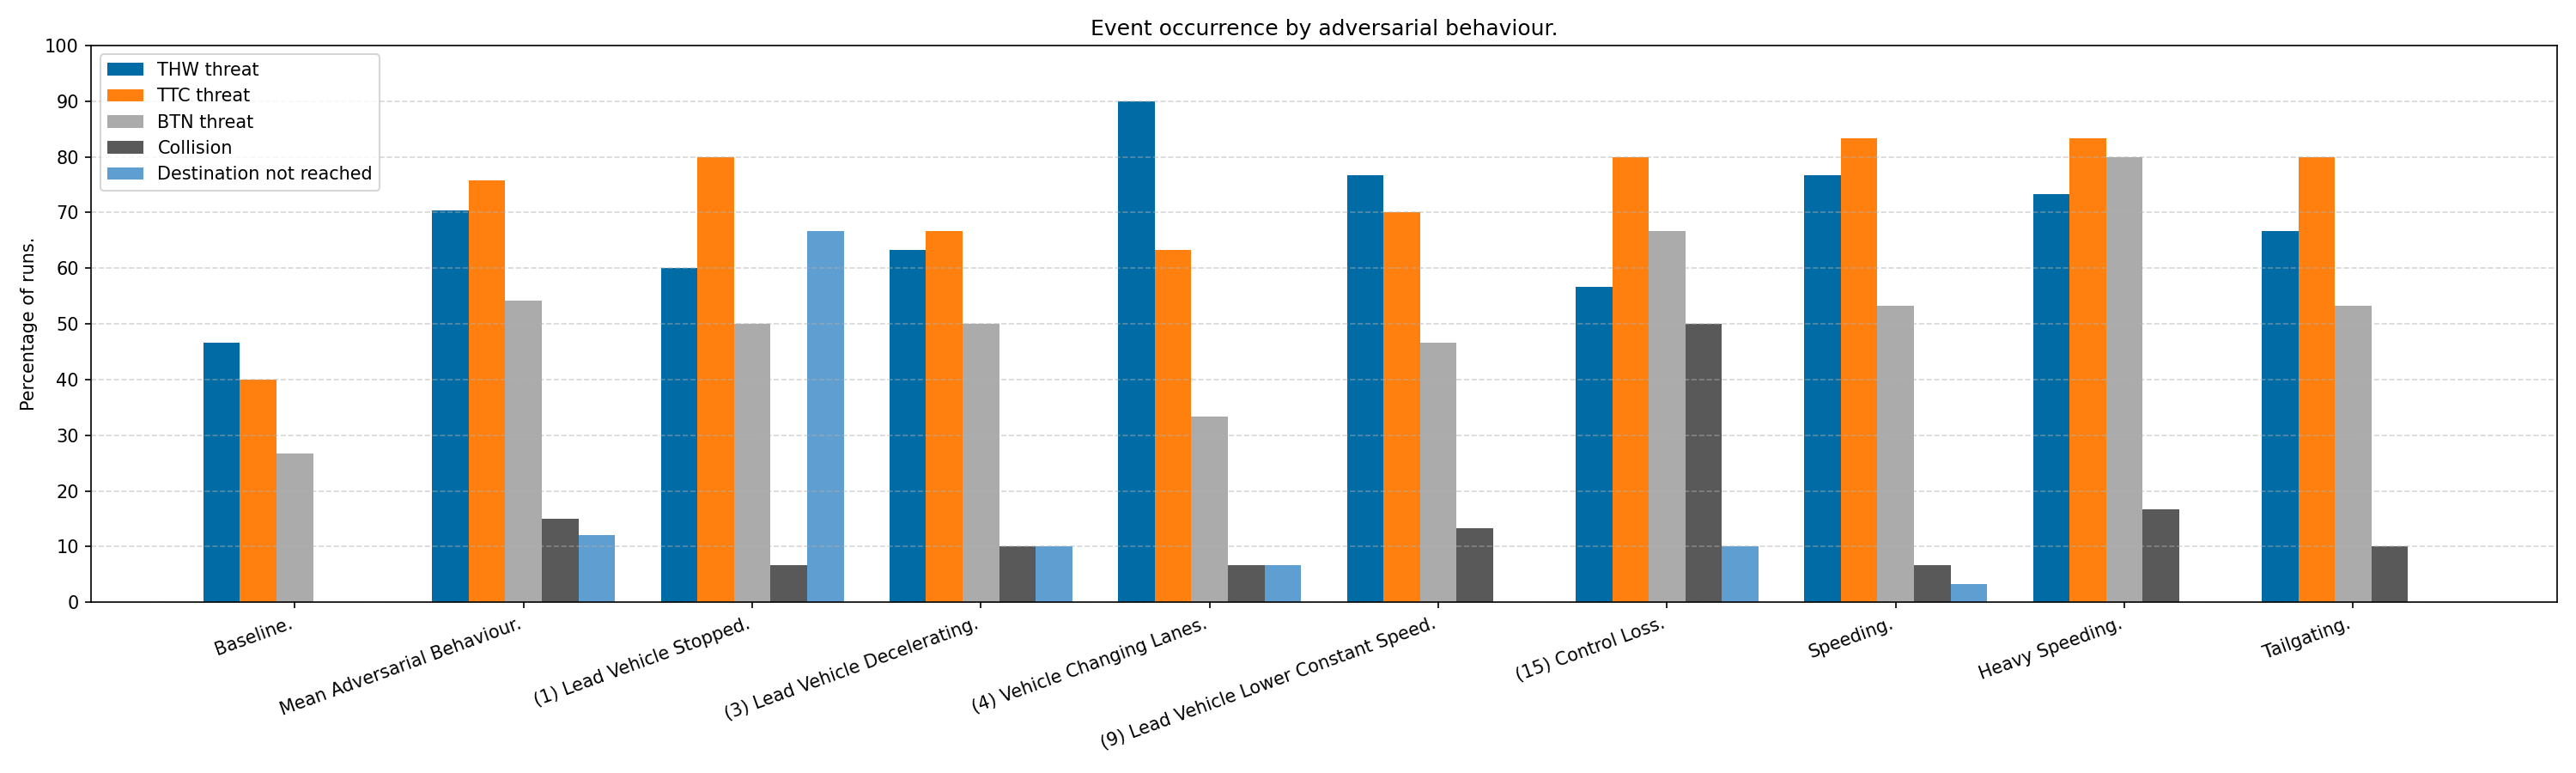
\includegraphics[width=1\linewidth]{imgs/rdb_events.png}
          \caption{Event occurrence by adversarial behaviour, roundabouts.}
          \label{fig:rdb_events}
\end{figure*}

\fi










\endinput
%%
%% End of file `sample-sigconf.tex'.
